I continue with presenting two very simple example methods that illustrate the motivation and benefit from using cached profiles.
This should provide the reader with an understanding how and why cached profiles can be beneficial for the performance of a Java Virtual Machine.
I will omit any implementation details on purpose as they will be discussed in Chapter \ref{c:implementation} in detail.
\\\\
Ideally, being able to reuse the profiles from previous runs should result in two main advantages:
\begin{enumerate}
  \item \textbf{Lower start-up time of the JVM:} Having information about the program flow already, the compiler can avoid gathering profiles and compile methods earlier.
  \item \textbf{Less Deoptimizations:} Since cache profiles get dumped at the end of a compilation, when using these profiles the compiler can already include all optimizations for all different method executions. Less uncommon traps need to be placed and less deoptimizations should occur.
\end{enumerate}
I'm using my implementation described in Chapter \ref{c:implementation} in CachedProfileMode 0 (see \ref{s:mode0}) on top of openJDK 1.9.0.
The measurements are done on a Dual-Core machine running at 2 GHz with 8GB of RAM. To measure the method invocation time I use hprof \cite{hprof} and the average of 10 runs. The evaluation process has been automated using a couple of python scripts. The error bars show the 95\% confidence interval.
\section{Example 1}
\label{s:ex1}
For this very first example, On-stack replacement has been disabled to keep the system simple and easy to understand.
\\
Example one is a simple class that invokes a method one hundred times. The method itself consists of a long running loop. The source code is shown in Listing \ref{l:nocompile}.
Since OSR is disabled and a compilation to level 3 is triggered after 200 invocations this method never leaves the interpreter. I call this run the \textit{Baseline}.
To show the influence of cached profiles I use a compiler flag to lower the compile threshold explicitly and, using the functionality written for this thesis, tell Hotspot to cache the profile.
In a next execution I use these profiles and achieve significantly better performance as one can see in Figure \ref{f:nocompile}.
This increase comes mainly from the fact that having a cached profile available allows the JVM to compile highly optimized code for hot methods earlier (at a lower threshold) since there is no need to gather the profiling information first.
\\
Since the example is rather simple neither the baseline nor the profile usage run trigger any deoptimization. This makes sense because after the first invocation, all the code paths of the method have been taken already and are therefore known to the interpreter and saved in the profile.
\begin{lstlisting}[float,caption=Simple method that does not get compiled,label=l:nocompile,language=Java]
class NoCompile {
    double result = 0.0;
    for(int c = 0; c < 100; c++) {
      result = method1(result);
    }
    public static double method1(double count) {
        for(int k = 0; k < 10000000; k++) {
            count = count + 50000;
        }
        return count;
   }
}
\end{lstlisting}
\begin{figure}[ht]
  \begin{center}
    \centering
    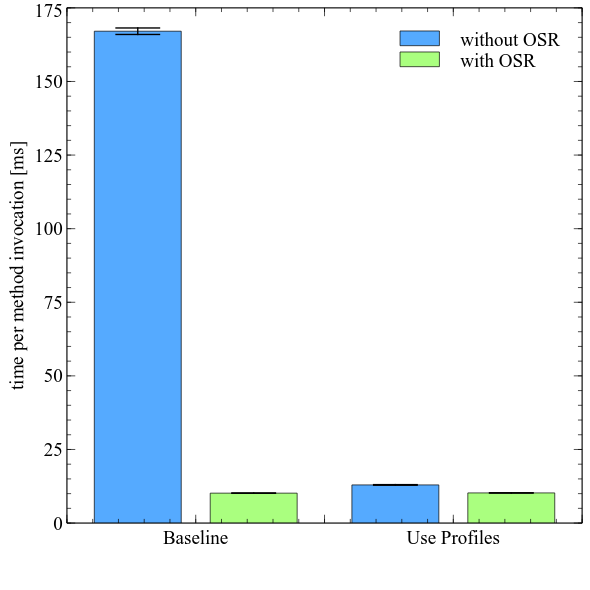
\includegraphics[width=0.5\textwidth]{figures/nocompile.png}
    \caption{NoCompile.method1 - per method invocation time}
    \label{f:nocompile}
  \end{center}
\end{figure}
\\\\
Enabling OSR again and the difference between with and without cached profiles vanishes.
This happens because Hotspot quickly realizes the hotness of the method and the JIT compiler produces perfectly optimized code during the first method invocation already. 
Even the OSR compiled code never triggers any deoptimization due to the simplicity of the loop.
So this example appears rather artificial since the same performance can be achieved with OSR already but nevertheless shows the influence of early compilation.
\section{Example 2}
\label{s:ex2}
However, OSR is one of the main features of Hotspot to improve the JIT performance and disabling that does not give us any practical results. Since we want an example which demonstrates the influence of cached profiles, I came up with the example sketched in Listing \ref{l:manydeopts} which is slightly more complex but still easy to understand.
\\\\
The idea is to create a method that takes a different, long running branch on each of it's method invocations. Each branch has been constructed in a way that it will trigger an OSR compilation. When compiling this method during its first iteration only the first branch will be included in the compiled code. The same will happen for each of the 100 method invocations. As one can see in Figure \ref{f:manydeopts} the baseline indeed averages at around 130 deoptimizations and a time per method invocation of 200 ms.
\\\\
Now I use a regular execution to dump the profiles and then use these profiles. So theoretically the profiles dumped after a full execution should include knowledge of all branches and therefore the compiled method using these profiles should not run into any deoptimizations. As one can see in Figure \ref{f:manydeopts} this is indeed the case. When using the cached profiles no more deoptimizations occur and because less time is spent profiling and compiling the methods the per method execution time is even significantly faster with averaging at 190ms now.
\begin{lstlisting}[float,caption=Simple method that causes many deoptimizations,label=l:manydeopts,language=Java]
class ManyDeopts {
    double result = 0.0;
    for(int c = 0; c < 100; c++) {
      result = method1(result);
    }
    public static long method1(long count) {
        for(int k = 0l; k < 10000000l; k++) {
            if (count < 10000000l) {
                count = count + 1;
            } else if (count < 30000000l) {
                count = count + 2;
                .
                .
                .
            } else if (count < 50500000000l) {
               count = count + 100;
            }
            count = count + 50000;
        }
        return count;
   }
}
\end{lstlisting}
\begin{figure}[ht]
  \begin{center}
    \centering
    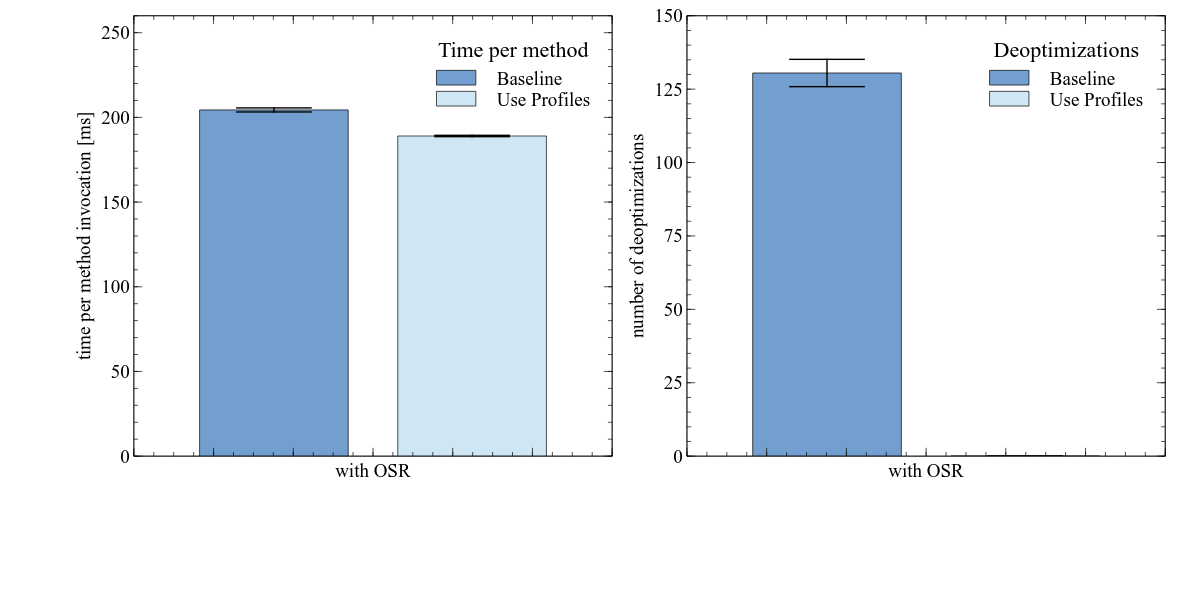
\includegraphics[width=0.9\textwidth]{figures/manydeopt.png}
    \caption{ManyDeopts.method1 - per method invocation time and deoptimization count}
    \label{f:manydeopts}
  \end{center}
\end{figure}
